\documentclass[12pt]{article}
\usepackage[utf8]{inputenc}
\usepackage{multicol}
\usepackage{graphicx}
\usepackage{amsmath}
\usepackage{amsfonts}
\usepackage{mathtools}
\usepackage{siunitx}
\usepackage{braket}
\usepackage{parskip}
\usepackage{wrapfig}
\usepackage[letterpaper, portrait, margin=1in]{geometry}
\renewcommand{\baselinestretch}{1.2}
\title{Quantum HW5}
\author{bellenchia}
\date{March 2019}
\begin{document}
\maketitle

\section*{The Classically Forbidden Region}
\subsection*{18.a)}
Represented in Hermite Polynomial form, the solutions of the Harmonic Oscillator are;\\

$\psi_n(x)=(\frac{m\omega}{\pi\hbar})^{\frac{1}{4}}\frac{(1}{\sqrt{2^nn!}}H_n(\xi)e^{-\xi^2/2}=(\frac{m\omega}{\pi\hbar})^{\frac{1}{4}}\frac{(-1)^n}{\sqrt{2^nn!}}(e^{\xi^2/2}\frac{d^n}{dx^n}[e^{-\xi^2/2}]e^{-\xi^2/2})$, with $\xi=\sqrt{\frac{m\omega}{\hbar}}x$\\


We want to evaluate the probability of finding the harmonic oscillator \textit{outside} the classical region (which is represented numerically as $E_n\leq V(x)$) \textbf{for the first ten states}.\\

We solve for the intersections; $ \frac{m\omega^2 x_0^2}{2}=En=\hbar\omega(n+\frac{1}{2})\Rightarrow x_0=\pm\sqrt{ 2\hbar(n+\frac{1}{2})/m\omega }$\\

Thus, the probability of being outside this region is $P(n)=1-{\displaystyle{\int_{x_0}^{-x_0}}}|\psi_n(x)|^2dx$\\

Mathematica is possibly the only language with a function for Hermite Polynomials so it was the obvious choice, especially since they don't have to be renormalized every iteration.\\

The following Mathematica Notebook shows all pertinent calculations;\\

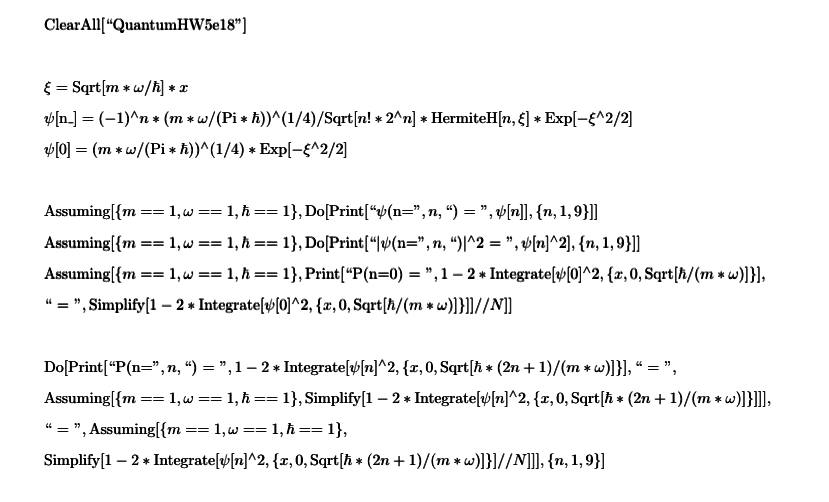
\includegraphics[width=\linewidth]{hw5ohmygod.png}
(The bounds cancel out any dependance on the parameters, so $\sqrt{m\omega/\hbar}=1$ is not necessary) .\\
{\small
\text{$\psi(n=0)=\frac{e^{-\frac{m x^2 \omega }{2 \hbar }} \left(\frac{m \omega }{\hbar }\right)^{1/4}}{\pi ^{1/4}}$}\\
\noindent\(\text{$\psi $(n=}1\text{) =  }-\frac{\sqrt{2} e^{-\frac{m x^2 \omega }{2 \hbar }} x \left(\frac{m \omega }{\hbar }\right)^{3/4}}{\pi ^{1/4}}\)

\noindent\(\text{$\psi $(n=}2\text{) =  }\frac{e^{-\frac{m x^2 \omega }{2 \hbar }} \left(-2+\frac{4 m x^2 \omega }{\hbar }\right) \left(\frac{m \omega
}{\hbar }\right)^{1/4}}{2 \sqrt{2} \pi ^{1/4}}\)

\noindent\(\text{$\psi $(n=}3\text{) =  }-\frac{e^{-\frac{m x^2 \omega }{2 \hbar }} \left(-12 x \sqrt{\frac{m \omega }{\hbar }}+8 x^3 \left(\frac{m
\omega }{\hbar }\right)^{3/2}\right) \left(\frac{m \omega }{\hbar }\right)^{1/4}}{4 \sqrt{3} \pi ^{1/4}}\)

\noindent\(\text{$\psi $(n=}4\text{) =  }\frac{e^{-\frac{m x^2 \omega }{2 \hbar }} \left(12+\frac{16 m^2 x^4 \omega ^2}{\hbar ^2}-\frac{48 m x^2
\omega }{\hbar }\right) \left(\frac{m \omega }{\hbar }\right)^{1/4}}{8 \sqrt{6} \pi ^{1/4}}\)

\noindent\(\text{$\psi $(n=}5\text{) =  }-\frac{e^{-\frac{m x^2 \omega }{2 \hbar }} \left(120 x \sqrt{\frac{m \omega }{\hbar }}-160 x^3 \left(\frac{m
\omega }{\hbar }\right)^{3/2}+32 x^5 \left(\frac{m \omega }{\hbar }\right)^{5/2}\right) \left(\frac{m \omega }{\hbar }\right)^{1/4}}{16 \sqrt{15}
\pi ^{1/4}}\)

\noindent\(\text{$\psi $(n=}6\text{) =  }\frac{e^{-\frac{m x^2 \omega }{2 \hbar }} \left(-120+\frac{64 m^3 x^6 \omega ^3}{\hbar ^3}-\frac{480 m^2
x^4 \omega ^2}{\hbar ^2}+\frac{720 m x^2 \omega }{\hbar }\right) \left(\frac{m \omega }{\hbar }\right)^{1/4}}{96 \sqrt{5} \pi ^{1/4}}\)

\noindent\(\text{$\psi $(n=}7\text{) =  }-\frac{e^{-\frac{m x^2 \omega }{2 \hbar }} \left(-1680 x \sqrt{\frac{m \omega }{\hbar }}+3360 x^3 \left(\frac{m
\omega }{\hbar }\right)^{3/2}-1344 x^5 \left(\frac{m \omega }{\hbar }\right)^{5/2}+128 x^7 \left(\frac{m \omega }{\hbar }\right)^{7/2}\right) \left(\frac{m
\omega }{\hbar }\right)^{1/4}}{96 \sqrt{70} \pi ^{1/4}}\)

\noindent\(\text{$\psi $(n=}8\text{) =  }\frac{e^{-\frac{m x^2 \omega }{2 \hbar }} \left(1680+\frac{256 m^4 x^8 \omega ^4}{\hbar ^4}-\frac{3584 m^3
x^6 \omega ^3}{\hbar ^3}+\frac{13440 m^2 x^4 \omega ^2}{\hbar ^2}-\frac{13440 m x^2 \omega }{\hbar }\right) \left(\frac{m \omega }{\hbar }\right)^{1/4}}{384
\sqrt{70} \pi ^{1/4}}\)

\noindent\(\text{$\psi $(n=}9\text{) =  }-\frac{e^{-\frac{m x^2 \omega }{2 \hbar }} \left(30240 x \sqrt{\frac{m \omega }{\hbar }}-80640 x^3 \left(\frac{m
\omega }{\hbar }\right)^{3/2}+48384 x^5 \left(\frac{m \omega }{\hbar }\right)^{5/2}-9216 x^7 \left(\frac{m \omega }{\hbar }\right)^{7/2}+512 x^9
\left(\frac{m \omega }{\hbar }\right)^{9/2}\right) \left(\frac{m \omega }{\hbar }\right)^{1/4}}{2304 \sqrt{35} \pi ^{1/4}}\)
}
\pagebreak


{\small
\noindent\(\text{P(n=0) = }1-\text{Erf}[1]\text{ = }0.157299\)

\noindent\(\text{P(n=}1\text{) = }1-\frac{\sqrt{\frac{m \omega }{\hbar }} \sqrt{\frac{\hbar }{m \omega }} \left(-2 \sqrt{\frac{3}{\pi }}+e^3 \text{Erf}\left[\sqrt{3}\right]\right)}{e^3}\text{
= }1+\frac{2 \sqrt{\frac{3}{\pi }}}{e^3}-\text{Erf}\left[\sqrt{3}\right]\text{ = }0.11161\)

\noindent\(\text{P(n=}2\text{) = }1-\frac{\sqrt{\frac{m \omega }{\hbar }} \sqrt{\frac{\hbar }{m \omega }} \left(-11 \sqrt{\frac{5}{\pi }}+e^5 \text{Erf}\left[\sqrt{5}\right]\right)}{e^5}\text{
= }1+\frac{11 \sqrt{\frac{5}{\pi }}}{e^5}-\text{Erf}\left[\sqrt{5}\right]\text{ = }0.0950694\)

\noindent\(\text{P(n=}3\text{) = }1-\frac{\sqrt{\frac{m \omega }{\hbar }} \sqrt{\frac{\hbar }{m \omega }} \left(-188 \sqrt{\frac{7}{\pi }}+3 e^7
\text{Erf}\left[\sqrt{7}\right]\right)}{3 e^7}\text{ = }1+\frac{188 \sqrt{\frac{7}{\pi }}}{3 e^7}-\text{Erf}\left[\sqrt{7}\right]\text{ = }0.0854829\)

\noindent\(\text{P(n=}4\text{) = }1-\frac{\sqrt{\frac{m \omega }{\hbar }} \sqrt{\frac{\hbar }{m \omega }} \left(-4533+4 e^9 \sqrt{\pi } \text{Erf}[3]\right)}{4
e^9 \sqrt{\pi }}\text{ = }1+\frac{4533}{4 e^9 \sqrt{\pi }}-\text{Erf}[3]\text{ = }0.0789264\)

\noindent\(\text{P(n=}5\text{) = }1-\frac{\sqrt{\frac{m \omega }{\hbar }} \sqrt{\frac{\hbar }{m \omega }} \left(-14213 \sqrt{\frac{11}{\pi }}+6 e^{11}
\text{Erf}\left[\sqrt{11}\right]\right)}{6 e^{11}}\text{ = }1+\frac{14213 \sqrt{\frac{11}{\pi }}}{6 e^{11}}-\text{Erf}\left[\sqrt{11}\right]\text{
= }0.0740342\)

\noindent\(\text{P(n=}6\text{) = }1-\frac{\sqrt{\frac{m \omega }{\hbar }} \sqrt{\frac{\hbar }{m \omega }} \left(-5494789 \sqrt{\frac{13}{\pi }}+360
e^{13} \text{Erf}\left[\sqrt{13}\right]\right)}{360 e^{13}}\text{ = }1+\frac{5494789 \sqrt{\frac{13}{\pi }}}{360 e^{13}}-\text{Erf}\left[\sqrt{13}\right]\text{
= }0.0701809\)

\noindent\(\text{P(n=}7\text{) = }1-\frac{\sqrt{\frac{m \omega }{\hbar }} \sqrt{\frac{\hbar }{m \omega }} \left(-2807901 \sqrt{\frac{15}{\pi }}+28
e^{15} \text{Erf}\left[\sqrt{15}\right]\right)}{28 e^{15}}\text{ = }1+\frac{2807901 \sqrt{\frac{15}{\pi }}}{28 e^{15}}-\text{Erf}\left[\sqrt{15}\right]\text{
= }0.0670313\)

\noindent\(\text{P(n=}8\text{) = }1-\frac{\sqrt{\frac{m \omega }{\hbar }} \sqrt{\frac{\hbar }{m \omega }} \left(-13478479397 \sqrt{\frac{17}{\pi
}}+20160 e^{17} \text{Erf}\left[\sqrt{17}\right]\right)}{20160 e^{17}}\text{ = }1+\frac{13478479397 \sqrt{\frac{17}{\pi }}}{20160 e^{17}}-\text{Erf}\left[\sqrt{17}\right]\text{
= }0.0643863\)

\noindent\(\text{P(n=}9\text{) = }1-\frac{\sqrt{\frac{m \omega }{\hbar }} \sqrt{\frac{\hbar }{m \omega }} \left(-408998132509 \sqrt{\frac{19}{\pi
}}+90720 e^{19} \text{Erf}\left[\sqrt{19}\right]\right)}{90720 e^{19}}\text{ = }1+\frac{408998132509 \sqrt{\frac{19}{\pi }}}{90720 e^{19}}-\text{Erf}\left[\sqrt{19}\right]\text{
= }0.0621191\)
}
\linebreak
\begin{center}
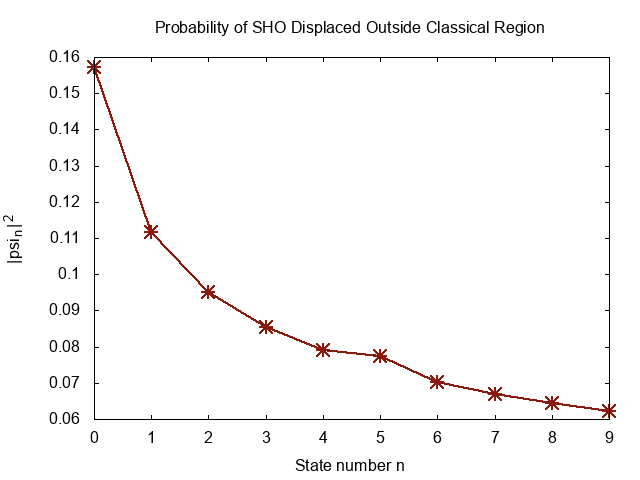
\includegraphics[width=0.8\textwidth]{proba2.png}\\
\end{center}

\subsection*{18b.)}
Evaluating the Schr$\ddot{\text{o}}$dinger equation for $V(x)>E$ yields the form; \\

$\psi(x)''=\sqrt{\frac{-2m(E-V(x))}{\hbar^2}}\psi(x)$. This creates a positive value under the square root sign. \\

In our previous cases with a constant potential, this implied our solution was of the form $\psi(x)=Ae^{kx}+Be^{-kx}$ \\ 

We see, as opposed to when $E\geq V$ and we obtained a complex exponential with sinusoidal behavior.\\

For the harmonic oscillator, this corresponds to similar behavior. Outside the classical region, there are no nodes because the form of the equation does not cross the x-axis.\\
%
%
%
\section*{19.) Half-Harmonic Oscillator}
 Suppose instead of the typical quadratic potential, there is an infinite potential in the other half region;\\

\[V(x)=
\begin{cases}
\infty & x<0 \\
m\omega^2x^2/2 & x\geq0
\end{cases}
\]\\

Griffith's text algebraically derives the solution to the Schr$\ddot{\text{o}}$dinger equation for a Harmonic Oscillator. This is done using the "Ladder Operators" $a_{\pm}=\frac{1}{\sqrt{2\hbar m\omega}}(m\omega x\mp ip)$, recall that $p=\frac{\hbar}{i}\frac{d}{dx}$.\\

This allows us to rewrite the Hamiltonian as $H=\hbar\omega(a_\pm a_\mp\pm\frac{1}{2})\psi$

Now, we can rewrite the equation as $\hbar\omega(a_\pm a_\mp\pm\frac{1}{2})\psi=E\psi$\\

These are likened to a ladder because repeatedly applying the raising/lowering operators to a given solution generates new solutions with differing energy levels, given by $E_n=\hbar\omega(n+\frac{1}{2})$. However, this becomes physically insignificant when achieving a negative energy.\\

We utilize the fact there must be one energy state $\psi_0$ such that $a_i\psi_0=0$, we will call this the "Ground State" and solve for the wavefunction appropriately;\\

$\frac{1}{\sqrt{2\hbar m\omega}}(m\omega x)\psi_0=-\hbar\omega\frac{d\psi_0}{dx}\Longrightarrow{\displaystyle\int_0^\infty}\frac{m\omega}{2\hbar}xdx=-{\displaystyle\int_0^\infty}\frac{d\phi_0}{\phi_0}$\\

$\Rightarrow ln|\phi_0|=(-\frac{m\omega}{2\hbar}x^2)+const.\Rightarrow\phi_0(x)=A e^{(-\frac{m\omega}{2\hbar}x^2)}$\\

Now we reach a problem, a clear boundary condition to be satisfied given such a potential is that $\psi_0(0)=0$. This means we can only accept \textit{odd} solutions for $\psi_n(x)=A_n(a_+)^n\psi_0(x)$, and to correct for the normalization constant we consider the fact odd functions have equal area under the curve about the central axis, and thus a factor of $\sqrt{2}$ must be introduced.\\

Thus, our steady state solutions with energy spacing  $\Delta E=2\hbar\omega$ are as follows;\\
\[
\chi_{2n+1}(x)=
\begin{cases}
\sqrt{2}\phi_n(x) & x\geq0\\
0 & x<0
\end{cases} 
\]
\linebreak
\begin{wrapfigure}{r}{0.5\linewidth}
  \begin{center}
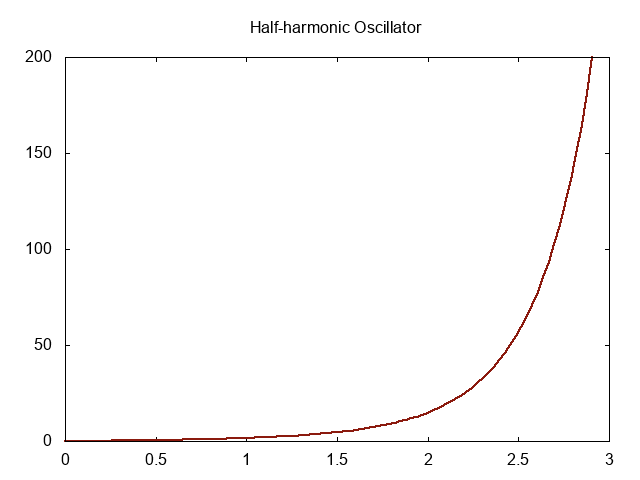
\includegraphics[width=0.4\textwidth]{hw5plot.png}
  \end{center}
\end{wrapfigure}

The ground state was plotted using the following GNUplot code;\\
set terminal png\\
set output 'hw5.png'\\
unset key\\
p(x)=x*exp(x**2/2)\\
plot p(x) w l ls 1\\
\pagebreak
\section*{20.) Heisenberg Picture}

We're given $\frac{da_H(t)}{dt}=\frac{i}{\hbar}[H,a_H(t)]$, and $\frac{da^\dagger_h(t)}{dt}=\frac{i}{\hbar}[H,a^\dagger_h(t)]$ for the SHO of frequency $\omega$\\

We will first employ some operator wizardry, multiplying the Hamiltonian by $1=e^{iHt/\hbar}e^{-iHt/\hbar}$, and since H commutes with any and all operators of itself;\\

$1\cdot H=e^{iHt/\hbar}e^{-iHt/\hbar}H=e^{iHt/\hbar}He^{-iHt/\hbar}$, now let's represent H in the form of raising and lowering operators; $H=\hbar\omega(a_s^\dagger a_s+\frac{1}{2}$) so we get;\\

$H=\hbar\omega e^{iHt/\hbar}(a^\dagger_s a_s +\frac{1}{2})e^{-iHt/\hbar}=\hbar\omega(e^{iHt/\hbar}a^\dagger_s a_se^{-iHt/\hbar})+\frac{1}{2}$\\

We can then insert another value of unity; $1=e^{-iHt/\hbar}e^{iHt/\hbar}$ between $a^\dagger_s$ and $ a_s$;\\

$H=\hbar\omega(e^{iHt/\hbar}a^\dagger_s e^{-iHt/\hbar} e^{iHt/\hbar} a_se^{-iHt/\hbar})+\frac{1}{2}$\\

Recognizing the relationship between Heisenberg and Schroedinger pictures\\

$a_h=e^{iHt/\hbar}a_se^{-iHt/\hbar}$ and $a^\dagger_h=e^{iHt/\hbar}a^\dagger_s e^{-iHt/\hbar}$, the same is true for $a^\dagger_h$\\

Finally, we see the hamiltonian can be written as $H=\hbar\omega(a_s^\dagger a_s+\frac{1}{2})$\\

Plug her back into the commutator; $\frac{da_h}{dt}=\frac{i}{\hbar}(\hbar\omega)[a_h,\hbar\omega(a^\dagger_s a_s +\frac{1}{2})]$ We can use the "Equal-time Commutation Relation," which states $[a_h,a^\dagger_h]=1$, the same as for $[a_s,a^\dagger_s]=1$\\

Note that all the relations we have shown are true in both $a_h$ and $a^\dagger_h$

$=\frac{i}{\hbar}(\hbar\omega)[a_h,a^\dagger_s a_s +\frac{1}{2}]=i\omega(a^\dagger_h[a_h,a_h]+[a_h,a^\dagger_h]a_h)=i\omega a_h$\\

$\Rightarrow \frac{d}{dt}a_h=i\omega a_h$, and then repeating the process for the second equation, we get\\ $\frac{d}{dt}a^\dagger_h=i\omega(a^\dagger_h[a^\dagger_h,a_h]+[a^\dagger_h,a^\dagger_h]a_h)=-i\omega a^\dagger_h$\\
\pagebreak

Now the final steps; we recognize that these are simple differential equations ;\\

$\frac{d}{dt}a_h(t)=i\omega a_h(t)$ and $\frac{d}{dt}a^\dagger_h(t)=-i\omega a^\dagger_h(t)$\\

Their solutions are of the form $a_h(t)=a_h(0)e^{i\omega t}$, and $a^\dagger_h(t)=a^\dagger_h(0)e^{-i\omega t}$\\

We employ their respective relations to the Schr$\ddot{\text{o}}$dinger picture;\\

$a_h(t)=e^{iHt/\hbar}a_s e^{-i\omega}$, and $a^\dagger_h(t)=e^{iHt/\hbar}a^\dagger_s e^{-i\omega}$\\

Plugging in $t=0$, $\Rightarrow a_h(0)=a_s$, $a^\dagger_h(0)=a^\dagger_s$ and thus, our solutions are\\
\linebreak

\begin{center}
{\huge   
    $a_h(t)=a_s e^{i\omega t}$\\
    
     $a^\dagger_h(t)=a^\dagger_s e^{-i\omega t}$\\
    }
\end{center}

\end{document}
